\documentclass[problem]{mcs}

\begin{pcomments}
  \pcomment{MQ_chi4}
  \pcomment{ARM 10/21/13}
\end{pcomments}

\pkeywords{
  coloring
  chromatic_number
}

%%%%%%%%%%%%%%%%%%%%%%%%%%%%%%%%%%%%%%%%%%%%%%%%%%%%%%%%%%%%%%%%%%%%%
% Problem starts here
%%%%%%%%%%%%%%%%%%%%%%%%%%%%%%%%%%%%%%%%%%%%%%%%%%%%%%%%%%%%%%%%%%%%%

\begin{problem}
Show that the chromatic number of the graph, $G$, below is four.

\begin{figure}[h]
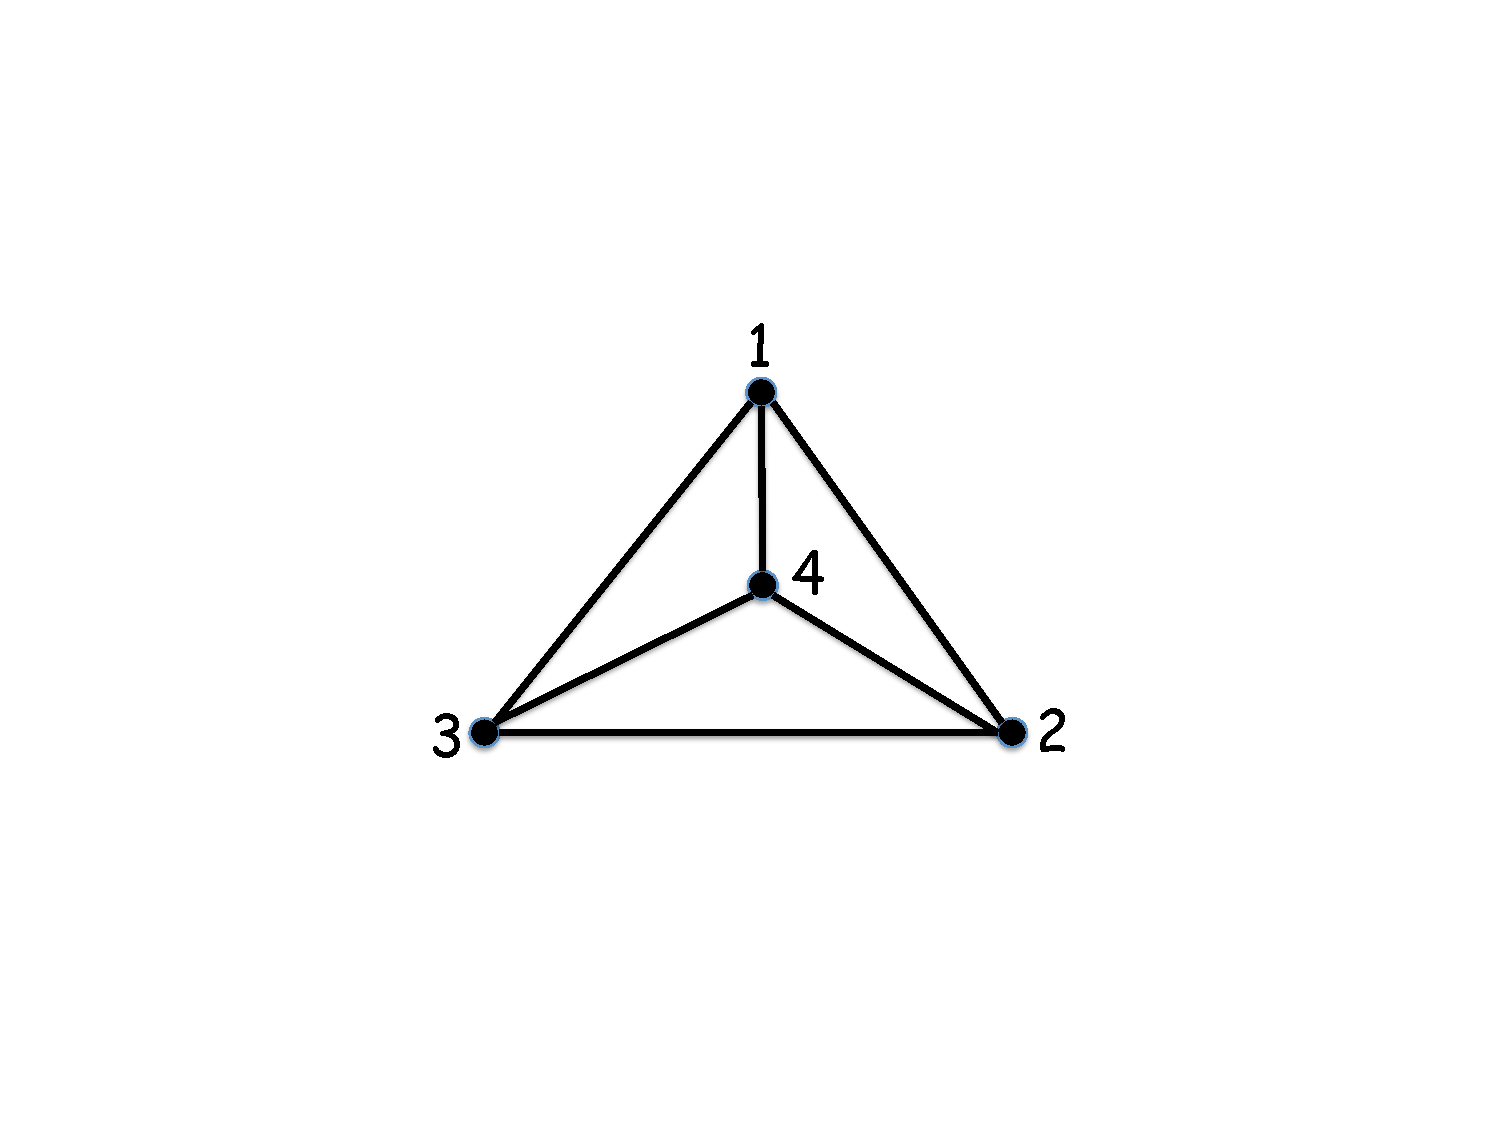
\includegraphics[width = 3in]{chi4}
\caption{Graph $G$ with $\chi(G)=4$.}
\end{figure}

\examspace[3in]

\begin{solution}
Since every two vertices are adjacent, all vertices must have
different colors.  There are four vertices, so $\chi(G)=4$.

Of course $G$ is the complete graph $K_4$, and it was already noted in
Section~\bref{sec:coloring} that $\chi(K_n) = n$.
\end{solution}

\end{problem}

\endinput
